% THESIS CHAPTER

\chapter{Control and state estimation}
\label{chap:fifth
}
\ifpdf
    \graphicspath{{Chapter5/Figures/PNG/}{Chapter5/Figures/PDF/}{Chapter5/Figures/}}
\else
    \graphicspath{{Chapter5/Figures/EPS/}{Chapter5/Figures/}}
\fi

% short summary of the chapter
\section*{Summary}
Due to the nature of the dynamics of the quadrotor, several control algorithms have been applied to it. As to be expected, each control scheme has its advantages and disadvantages. This chapter presents the techniques that are used to estimate the system's states and to stabilize IRIS which are currently implemented in the PX4 Firmware.\par After a quick overview of the estimator modules, the controller architecture is presented. Moreover, this chapter explains in details how the on board autopilot interfaces with the software architecture and which modules are involved.

\section{Introduction to the PX4 Flight Stack}

The PX4 Flight Stack denotes the list of all the applications running on board the PixHawk. Those modules provide the services and methods which are necessary to manage the radio communications, inter process message pass-through, data logging, state estimation, control, high level states and low level communication with motors and sensors.

\subsection{Message pass-through}
The core on board applications are started at system startup, others can be started via the NuttShell or forced to startup by inserting them in the start boot file. Every application runs independently with its own frequency; the interfaces between processes are managed by \textit{uOrb} middleware (Micro Orb) which, with the use of topics, guarantees the message pass-through for data packets over named buses. Those topics encode structs and they are pre defined. In PX4, a topic (often called node) contains only one message type, e.g. the \textit{vehicle attitude} topic transports a message containing the attitude struct (roll, pitch and yaw estimates).\par Nodes can publish a message on a bus/topic or subscribe to a bus/topic. They are not aware of who they are communicating with. There can be multiple publishers and multiple subscribers to a topic (Figure \ref{figure:pubsub}). This design pattern prevents locking issues and is very common in robotics. \textbf{To make this efficient, there is always only one message on the bus and no queue is kept} \cite{uOrb}. The total list of \textit{uOrb} topics can be found in the uOrb folder of the PX4 Firmware since the online documentation is not updated. \\

\noindent
The external communication (through radio link) is managed by mavlink, previously presented in section \ref{sec:mavlink}, however Mav packets are translated in uOrb topics internally.   

\begin{figure}[h]
	\centering
	\noindent
	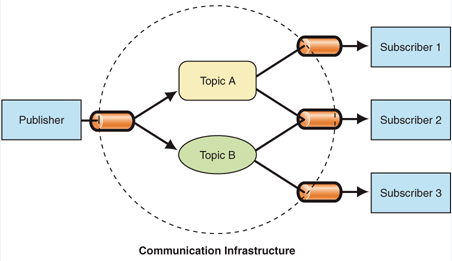
\includegraphics[width=0.6\textwidth]{pub_sub.PNG}
	\caption{Publish/Subscribe design pattern}
	\label{figure:pubsub}
\end{figure}

\subsection{Onboard nodes}


The most relevant apps that are started at boot can be divided in groups. \\

\noindent
\paragraph{System applications} Those kind of nodes manage the internal and external process communications , logging and testing. They provide the basic services on which the other modules rely:	
\begin{itemize}
	\item mavlink - is dedicated to pack and unpack mavlink messages.
	\item sdlog2 - takes relevant topics and creates a log file on sd card at every flight.
	\item test - mainly used for troubleshooting.
	\item uOrb - inter-process communication middleware .
\end{itemize}
\paragraph{Drivers} As one may imagine, those nodes represent the layer between hardware and software. They manage the communication with sensors, ports and buses:
\begin{itemize}
	\item esc\_calib - calibration of the electronic speed controllers for motors.
	\item fmu - manages the board input and output pins.
	\item GPS - GPS reciever driver
	\item pwm - command the pwm to be sent to motor controllers
	\item sensor - communication with various sensors (inertial, baro)
\end{itemize}
\paragraph{Attitude and position estimators} Those modules are responsible for position and attitude estimation, they are part of the core of the flight stack:
\begin{itemize}
	\item position\_estimator\_inav - estimates position with inertial sensor, gps and mocap measuraments.
	\item att\_estimator\_ekf - estimates attitude using inertial sensors.
\end{itemize}
\paragraph{Multirotor Attitude and Position Controllers} Those are the key modules regarding this thesis. They implements the algorithms for position and attitude control:
\begin{itemize}
	\item mc\_pos\_control - position controller
	\item mc\_att\_control - attitude controller
\end{itemize}

\paragraph{Flight safety and navigation} Those are the key modules regarding this thesis. They implements the algorithms for position and attitude control:
\begin{itemize}
	\item commander - internal state machine which determine system states for safety (flying, idle , emergency , on ground)
	\item navigator - highest level of abstraction, it implements mission following and failsafe
\end{itemize}

\subsection{State machine overview}

The system relies on a state machine in order to manage what it can and cannot do at a particular moment. The main task of this module is to assure safety from an high level point of view. Other safety procedures are implemented also on a lower level on hardware. \\

\noindent
The main states are \textit{ARMED , STAND-BY , INIT , ERROR} and \textit{UNLOCKED}. At the moment the user turns on the robot, the state machine is in \textit{INIT} state. Here all the procedure for sensor initialization and checklists are done. The next state then becomes \textit{STAND-BY} where IRIS waits for orders. By manually pressing a safety button, the state changes to UNLOCKED and back to STAND-BY by pressing again the button. In UNLOCKED state, the motor are electrically connected to the power source thus they can be armed. With a button on the remote control, the motors are armed and start spinning with idle velocity and the robot can fly. From any state, an error signal may arrive changing the actual configuration to ERROR. Here the motors are turned off after the automatic landing procedure and the robot must be rebooted. Those concept are depicted in figure \ref{figure:iris_state}.

\begin{figure}[h]
	\centering
	\noindent
	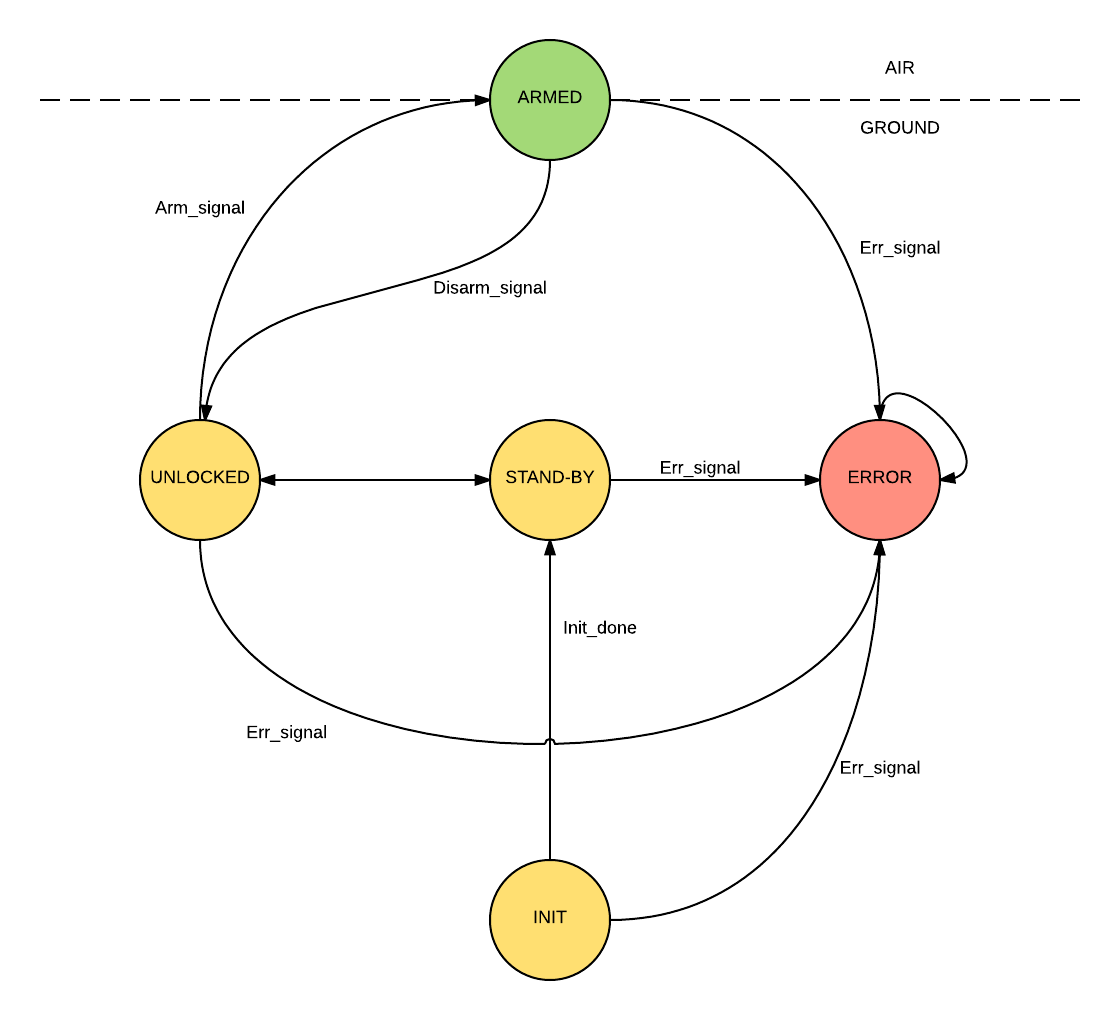
\includegraphics[width=0.7\textwidth]{iris_state.png}
	\caption{IRIS state machine}
	\label{figure:iris_state}
\end{figure}


\section{Estimation modules}

Since I am using an older version of PX4 because it is stable and well tested, the estimation occurs in two different modules. The first module, called \textit{position\_estimator\_inav} , is used to estimate the position of the quadcopter while the second, named\textit{ att\_estimator\_ekf }, estimates the attitude. The choice of dividing in two different processes the estimation phase  is mainly because attitude has an higher dynamics than position, this gives the possibility to run the attitude estimator at a frequency higher than the position estimator thus having better results.

\subsection{Position estimator}

The position estimator is based on inertial model and optimized for multirotors. It reads multiple sensors and estimates 3D position and velocity, in local and global frames. It is a fixed gain estimator and it relies on the following sources with the respective gains:
\begin{table}[H]
		\centering
	\begin{tabular}{l l r}
		\textbf{Sensor} & \textbf{ID} & \textbf{Gain} \\ \hline
		Accelerometer (for altitude) & INAV\_W\_Z\_ACC & 50 \\
		Barometer (gives absolute altitude)  & INAV\_W\_Z\_BARO & 50  \\
		Accelerometer (for x and y) & INAV\_W\_XY\_ACC & 10 \\
		GPS Position & INAV\_W\_XY\_GPS\_P & 1 \\
		GPS Velocity & INAV\_W\_XY\_GPS\_V & 2 \\
		Mocap estimate ( altitude ) & INAV\_W\_Z\_VIS\_P & 5 \\
		Mocap estimate ( altitude ) & INAV\_W\_XY\_VIS\_P & 7 \\
	\end{tabular}
\end{table}
%CORREGGI VALORI GUADAGNI
 




